\documentclass[a4paper,11pt,openright]{report}
\setlength{\parindent}{0pt} % set noindent for entire file

\usepackage[utf8]{inputenc}
\usepackage[a4paper,top=25mm,bottom=25mm,left=15mm,right=20mm]{geometry}
\usepackage{xcolor,graphicx}
\usepackage{amsmath}
\usepackage{setspace}
\usepackage{sectsty}
\usepackage{etoolbox}
\usepackage{enumitem}
\usepackage{listings}
\usepackage{textcmds}
\usepackage{times}

\graphicspath{ {/home/saran/Analytics/Jun_30/} }

\lstdefinestyle{mystyle}{
	backgroundcolor=\color{white},
	basicstyle=\ttfamily\footnotesize,
	breakatwhitespace=false,
	breaklines=true,
	captionpos=b,
	keepspaces=true,
	showspaces=false,
	showstringspaces=false,
	showtabs=false,
	tabsize=4
}

\lstset{style=mystyle}

\begin{document}
\singlespacing
\pagestyle{plain}

\begin{small}
\begin{center}
\textbf{Assignment: CRUD Operations} \\
Date: 07/10/2020 \hspace{2mm} Name: D.Saravanan
\end{center}
\end{small}

\vspace{10px}

\begin{footnotesize}
1. Create a collection, insert 6 documents, perform all the CRUD operations and display the
output.
\end{footnotesize}

{\footnotesize Insert}
%figure_1
\begin{figure}[ht!]
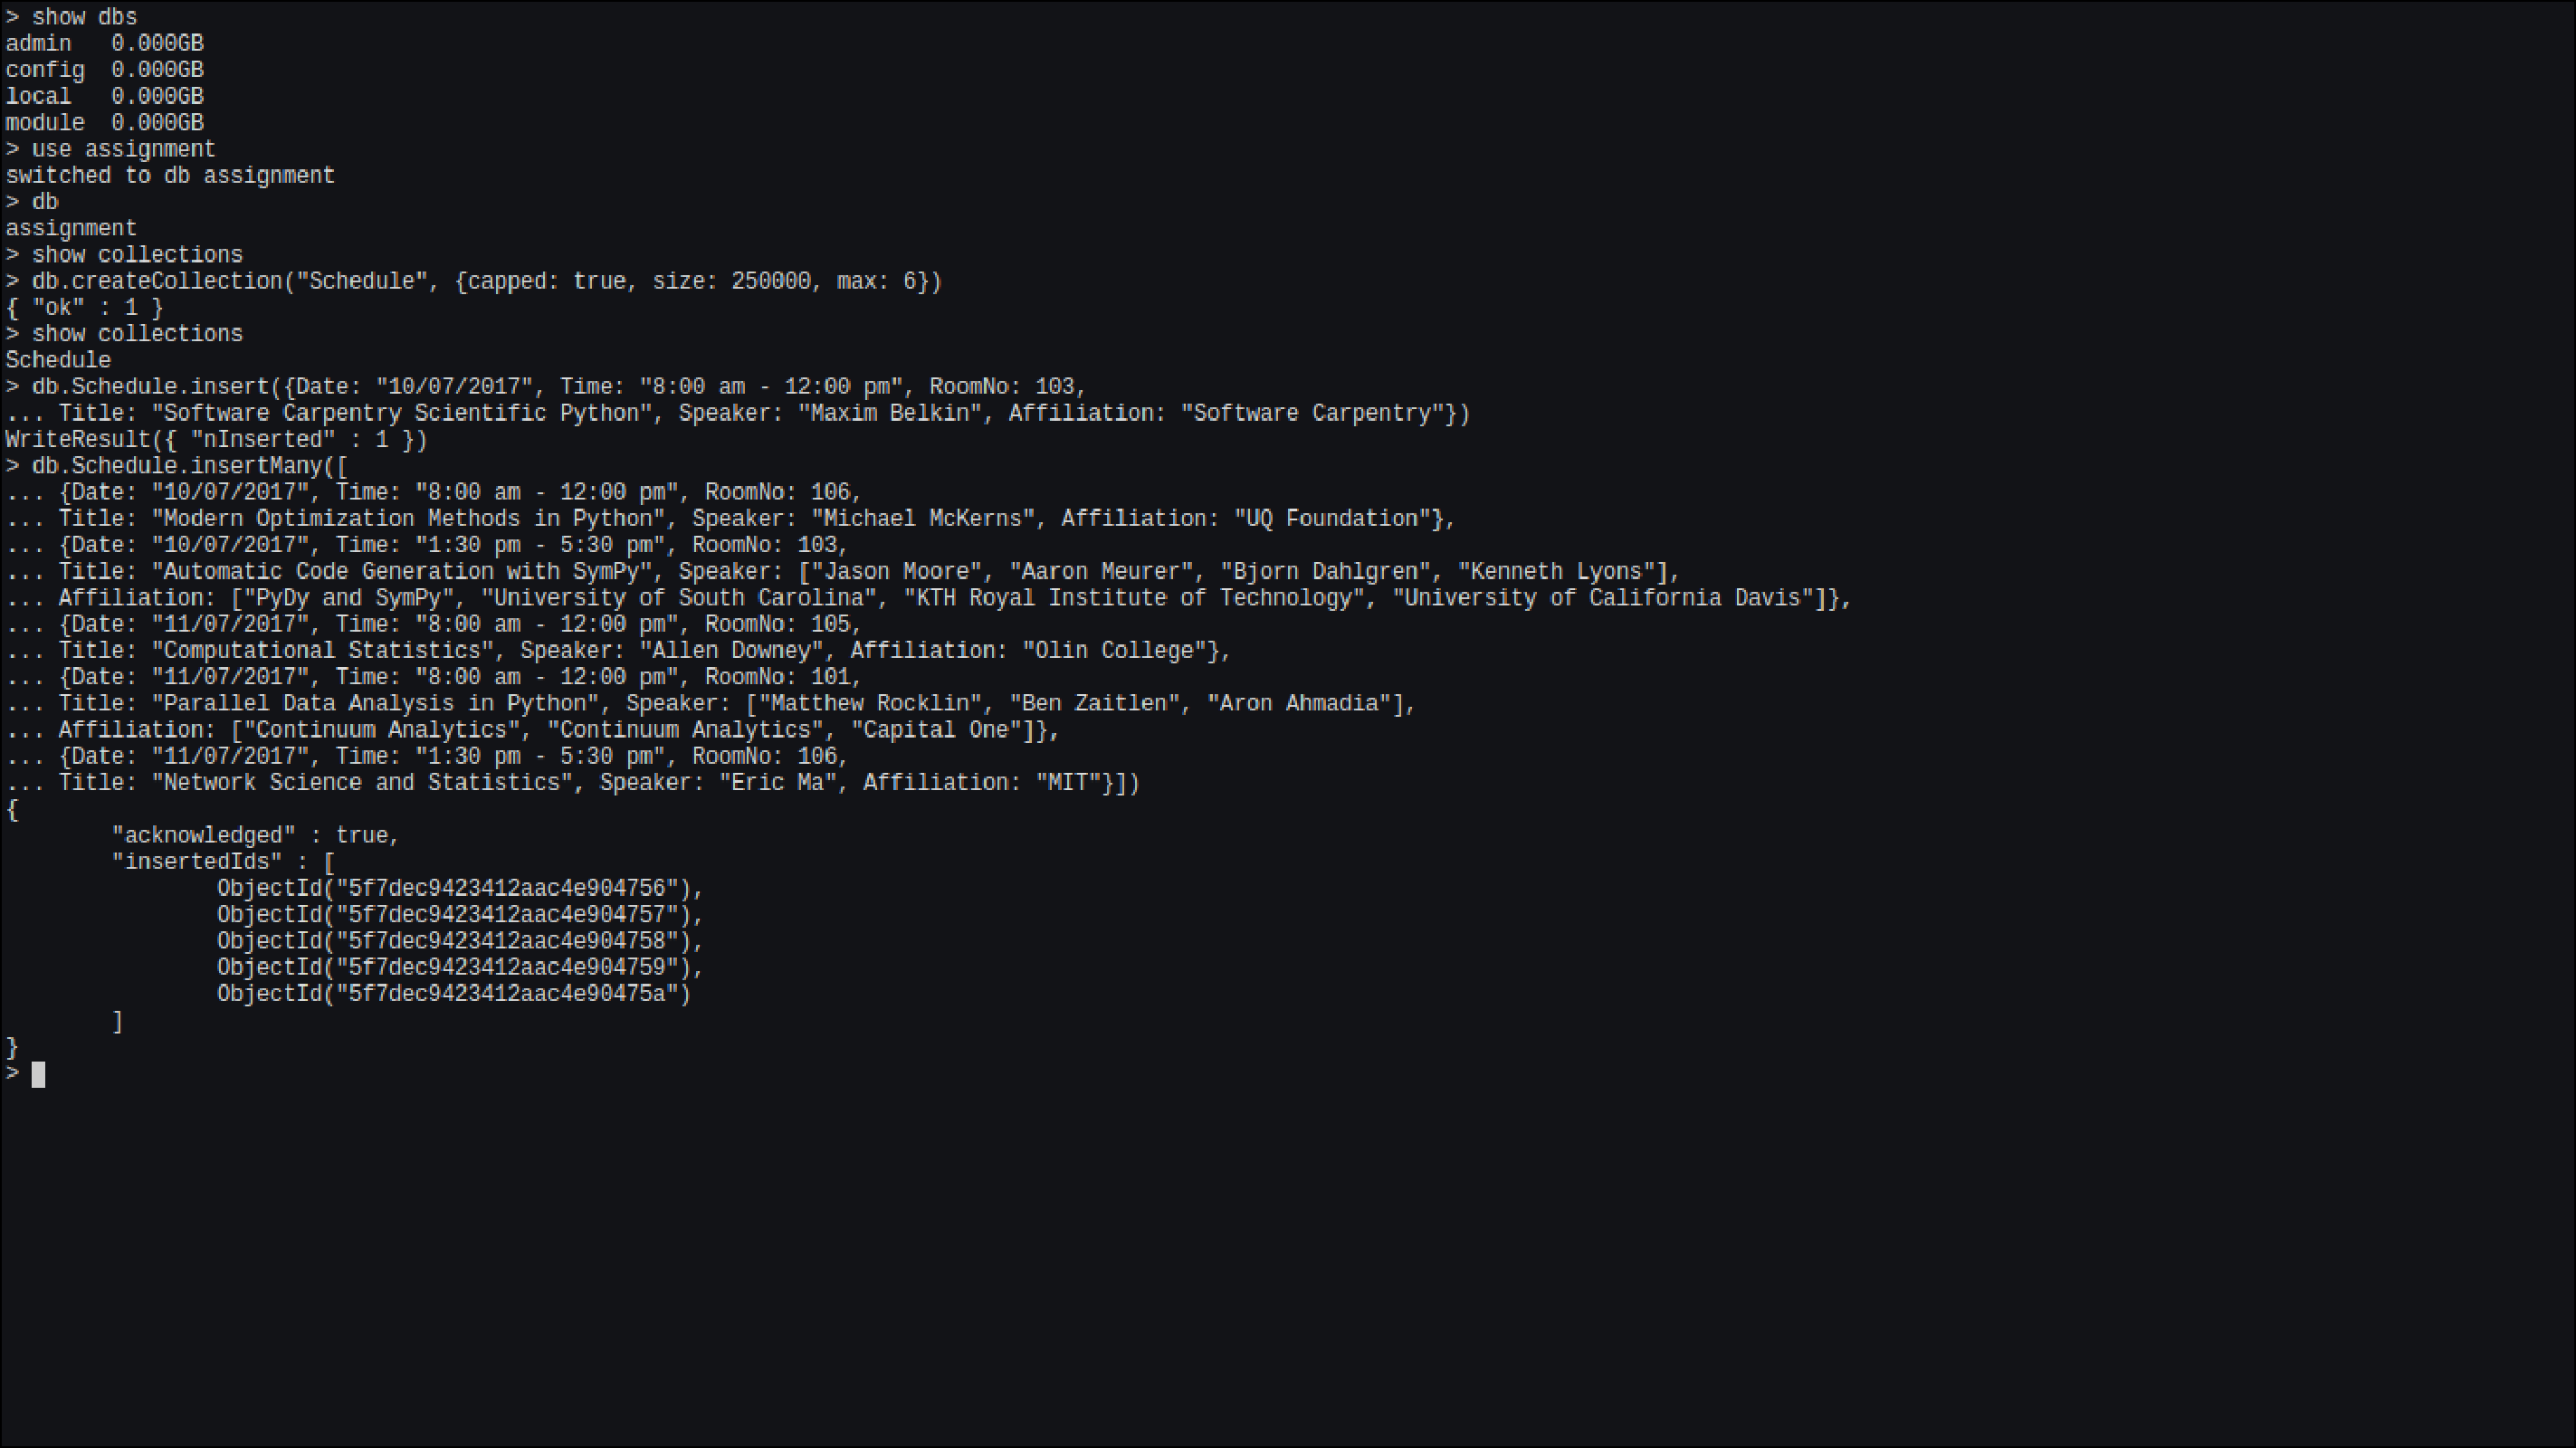
\includegraphics[width=20cm,height=10cm,keepaspectratio]{image1.pdf}
\centering
\end{figure}

{\footnotesize Query and Projection}
%figure_2
\begin{figure}[ht!]
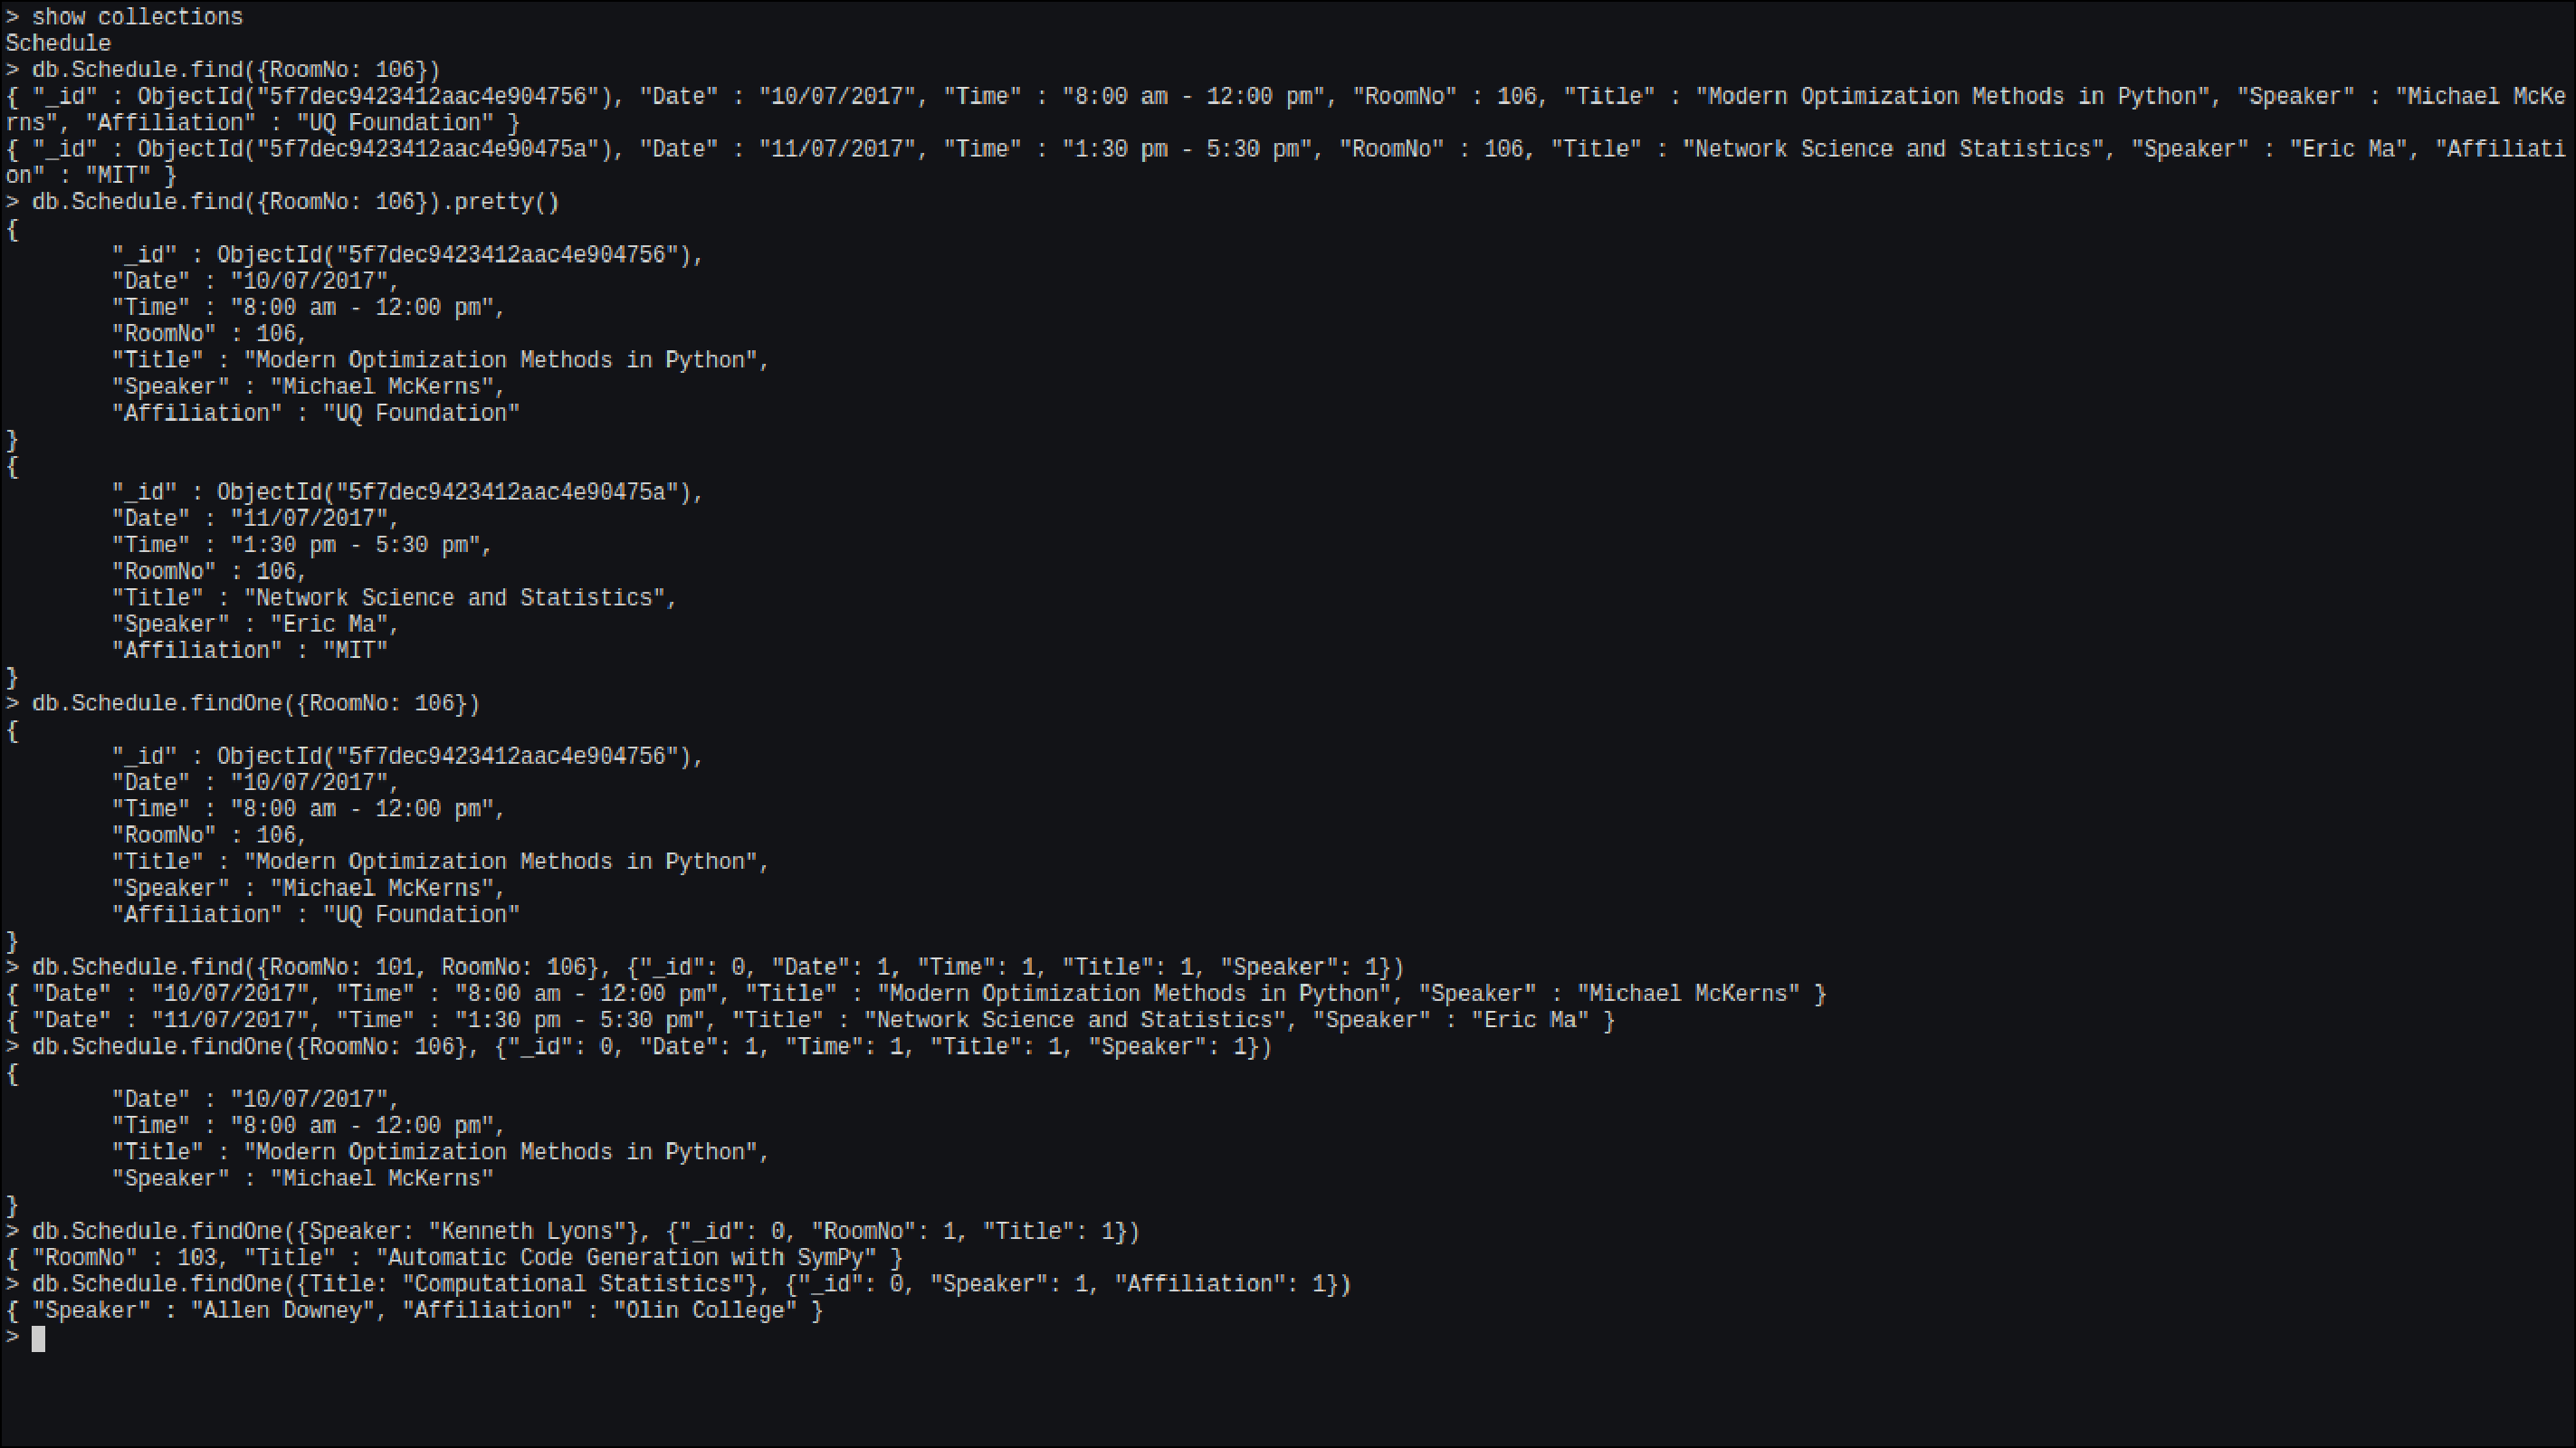
\includegraphics[width=20cm,height=10cm,keepaspectratio]{image2.pdf}
\centering
\end{figure}

\pagebreak

{\footnotesize Update}
%figure_3
\begin{figure}[ht!]
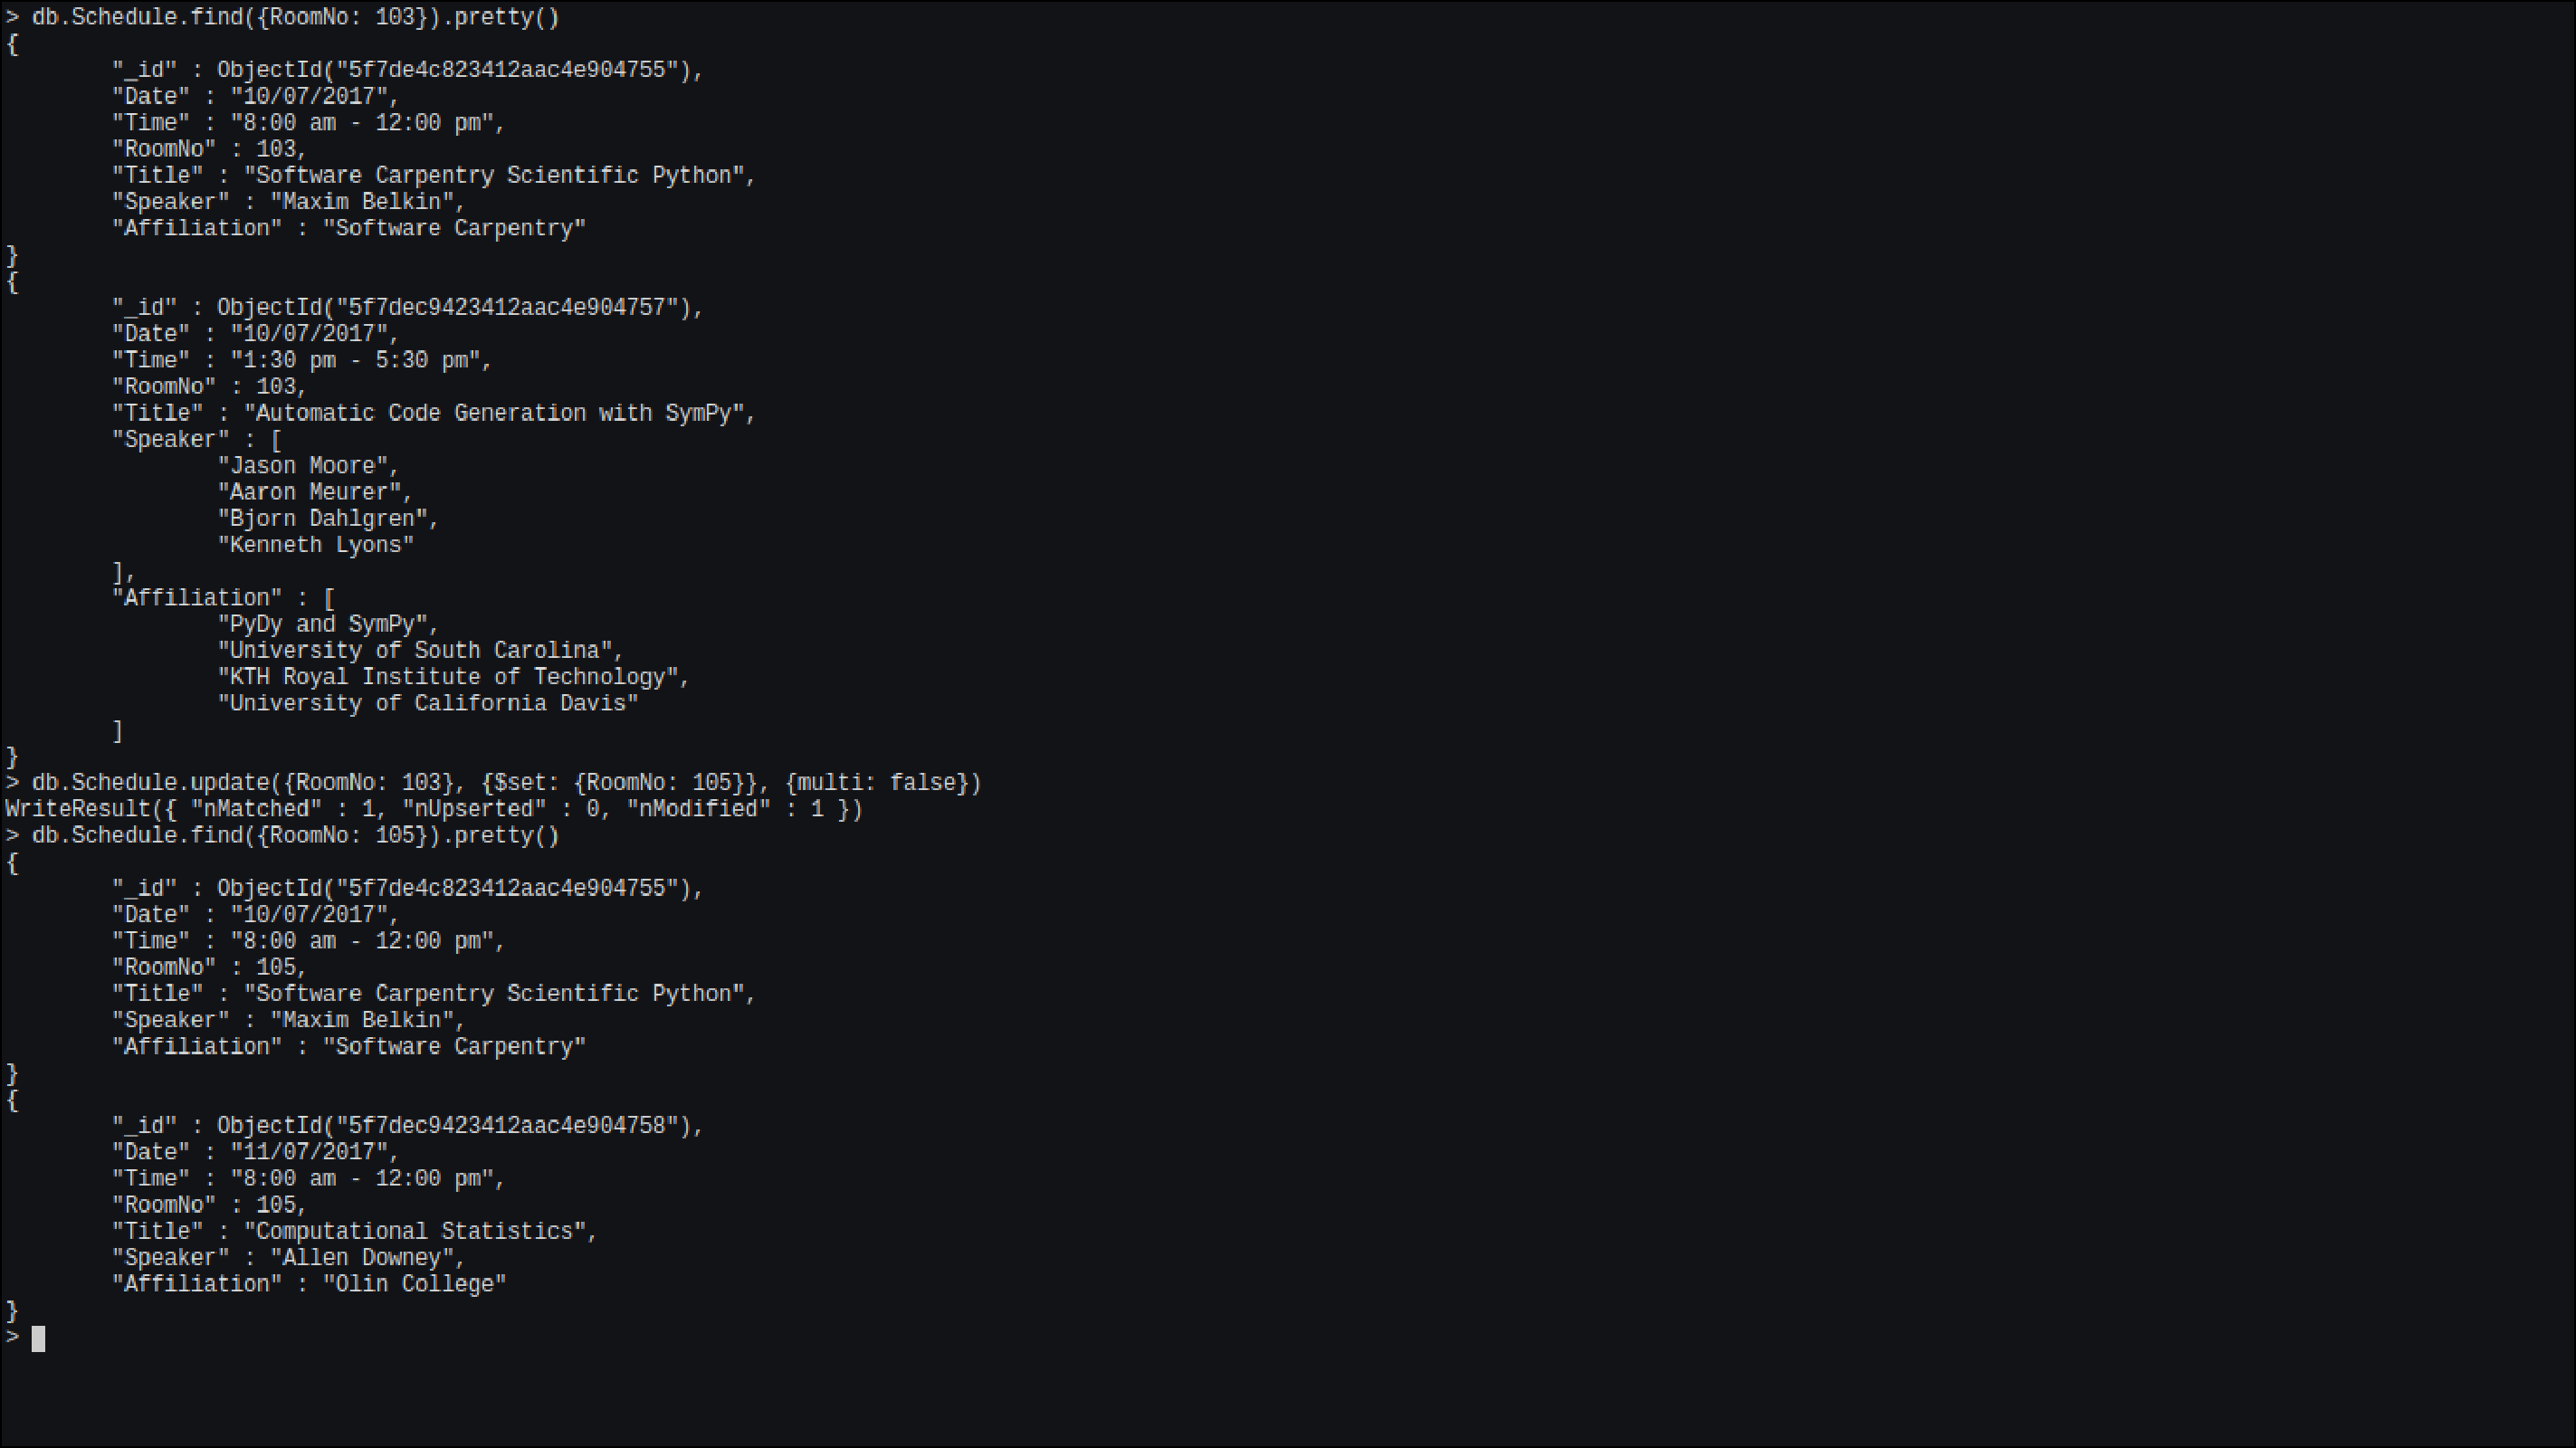
\includegraphics[width=20cm,height=10cm,keepaspectratio]{image3.pdf}
\centering
\end{figure}

\vspace{20px}

{\footnotesize Delete}
%figure_4
\begin{figure}[ht!]
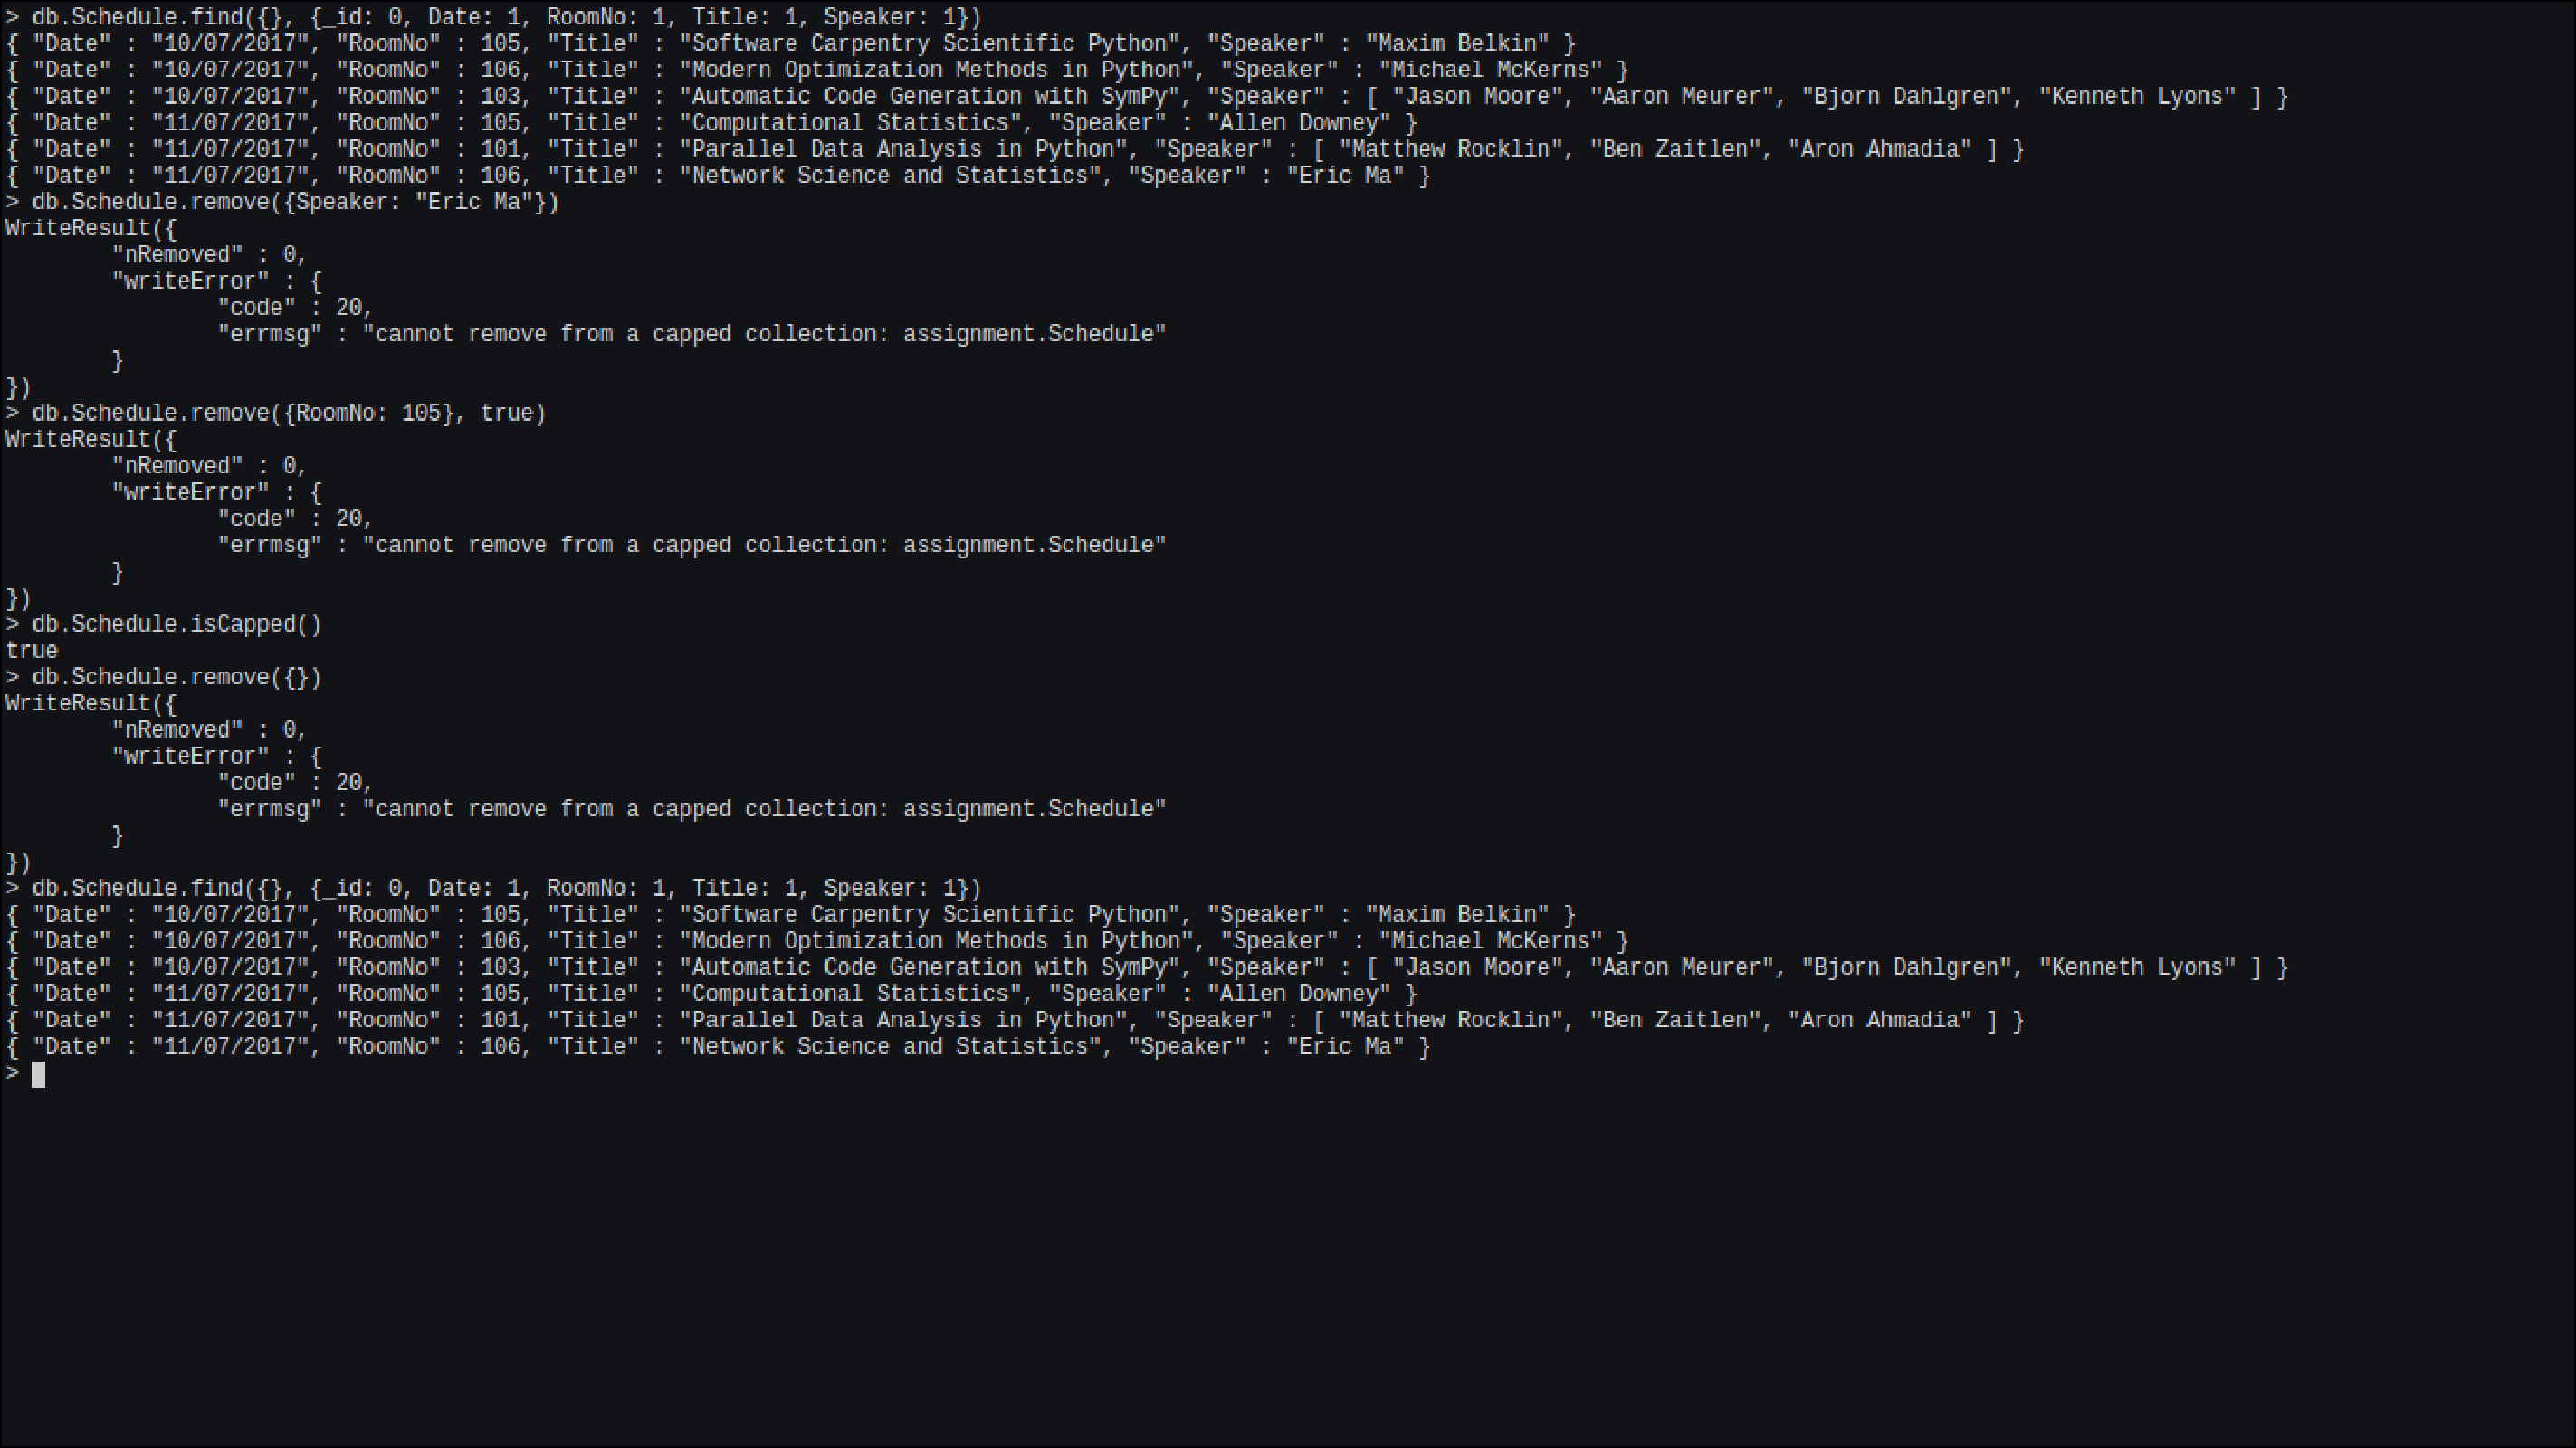
\includegraphics[width=20cm,height=10cm,keepaspectratio]{image4.pdf}
\centering
\end{figure}

\end{document}
